% ------------------------------------------------------------------------------
% TYPO3 Version 10.3 - What's New (Serbian Version)
%
% @license	Creative Commons BY-NC-SA 3.0
% @link		https://typo3.org/help/documentation/whats-new/
% @language	Serbian
% ------------------------------------------------------------------------------

\section{Izmene za integratore}
\begin{frame}[fragile]
	\frametitle{Izmene za integratore}

	\begin{center}\huge{Poglavlje 2:}\end{center}
	\begin{center}\huge{\color{typo3darkgrey}\textbf{Izmene za integratore}}\end{center}

\end{frame}

% ------------------------------------------------------------------------------
% Feature | 90333 | Dashboard

\begin{frame}[fragile]
	\frametitle{Izmene za integratore}
	\framesubtitle{Dashboard}

	% decrease font size for code listing
	\lstset{basicstyle=\tiny\ttfamily}

	\begin{itemize}
		\item Dashboard \textit{preseti} se mogu konfigurisati za nove korisnike
		ili za korisnike koji su izbrisali sve svoje dashboard-e.
		\item Ovo se može iskoristiti da se prikaže "Getting Started" dashboard kao podrazumevan.
		\item Primer TSconfig:

\vspace{-0.4cm}
\begin{lstlisting}
options.dashboard.dashboardPresetsForNewUsers = default, dashboardPreset-myPreset
\end{lstlisting}

		\item Više dashboard preseta se može definisati kao lista razdvojena zarezom.

	\end{itemize}

\end{frame}

% ------------------------------------------------------------------------------
% Important | 89992 | Use New TranslationServer

\begin{frame}[fragile]
	\frametitle{Izmene za integratore}
	\framesubtitle{Platforma za upravljanje prevodima}

	\begin{itemize}
		\item SaaS rešenje "\href{https://crowdin.com/}{Crowdin}" se od sada koristiti
			za upravljanje lokalizacijama/prevodima u TYPO3 platformi.
		\item Ohrabrujemo sve da uzmu učešće u ovome i unapredimo zajedno lokalizaciju.
		\item Crowdin se može koristiti za prevod labela iz jezgra TYPO3,
			kao i za prevod TYPO3 proširenja.
		\item Više možete pročitati u
			\href{https://docs.typo3.org/m/typo3/reference-coreapi/master/en-us/ApiOverview/Internationalization/TranslationServer/Crowdin.html}{TYPO3 dokumentaciji}.
	\end{itemize}

	\begin{figure}
		
\includegraphics[width=0.40\linewidth]{ChangesForIntegrators/crowdin-logo.png}
	\end{figure}

\end{frame}

% ------------------------------------------------------------------------------
% Feature | 90266 | Fluid-based templated emails

\begin{frame}[fragile]
	\frametitle{Izmene za integratore}
	\framesubtitle{HTML mejlovi zasnovani na Fluidu (1)}

	% decrease font size for code listing
	\lstset{basicstyle=\smaller\ttfamily}

	\begin{itemize}
		\item TYPO3 od sada podržava slanje mejlova kao HTML i kao čist tekst.
		\item Mejlovi se prave korišćenjem Fluid templating engin-a.
		\item Šabloni mejlova se mogu prilagoditi prepisivanjem putanja do fajlova:

\vspace{-0.4cm}
\begin{lstlisting}
$GLOBALS['TYPO3_CONF_VARS']['MAIL']['templateRootPaths'][700] =
  'EXT:my_site_extension/Resources/Private/Templates/Email';

$GLOBALS['TYPO3_CONF_VARS']['MAIL']['layoutRootPaths'][700] =
  'EXT:my_site_extension/Resources/Private/Layouts';
\end{lstlisting}

	\end{itemize}

\end{frame}

% ------------------------------------------------------------------------------
% Feature | 90266 | Fluid-based templated emails

\begin{frame}[fragile]
	\frametitle{Izmene za integratore}
	\framesubtitle{HTML mejlovi zasnovani na Fluidu (2)}

	\begin{itemize}
		\item HTML mejlovi zasnovani na Fluidu se koriste za sledeće komponente:

			\begin{itemize}
				\item Install Tool test mejl (primer na sledećem slajdu).
				\item Workspace obaveštenje o izmeni stanja.
				\item Mejl obaveštenja o logovanju korisnika na administratoriski interfejs.
			\end{itemize}

	\end{itemize}

\end{frame}

% ------------------------------------------------------------------------------
% Feature | 90266 | Fluid-based templated emails

\begin{frame}[fragile]
	\frametitle{Izmene za integratore}
	\framesubtitle{HTML mejlovi zasnovani na Fluidu (3)}

	Test mejl poslat putem Install Tool-a:

	\begin{figure}
		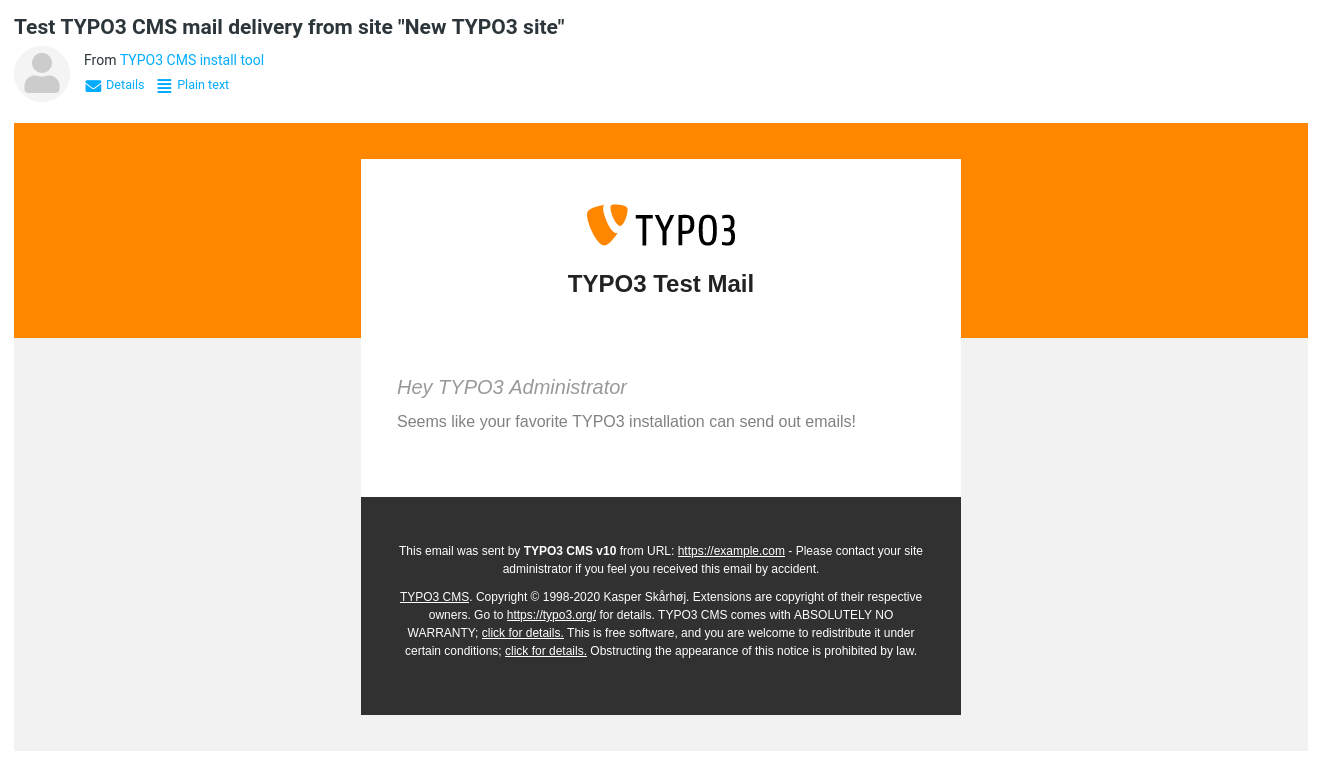
\includegraphics[width=0.8\linewidth]{ChangesForIntegrators/90266-FluidBasedTemplatedEmails.png}
	\end{figure}

\end{frame}

% ------------------------------------------------------------------------------
% Feature | 90203 | Make workspace available in TypoScript conditions

\begin{frame}[fragile]
	\frametitle{Izmene za integratore}
	\framesubtitle{Workspaces i TypoScript}

	% decrease font size for code listing
	\lstset{basicstyle=\smaller\ttfamily}

	\begin{itemize}
		\item Uvedena je nova jezička promenljiva: \texttt{workspace}.
		\item Ova promenljiva se može koristiti za uparivanje datog izraza sa
			parametrima workspace-a.
		\item Sledeći parametri su trenutno podržani:\newline
			\small
				\texttt{workspaceId}, \texttt{isLive}, i \texttt{isOffline}.
			\normalsize
		\item Na primer:

\vspace{-0.4cm}
\begin{lstlisting}
[workspace.workspaceId === 3]
  # Current workspace ID is 3
[end]
\end{lstlisting}

	\end{itemize}

\end{frame}

% ------------------------------------------------------------------------------
% Feature | 88962 | Re-implement old PIDupinRootline TypoScript condition

\begin{frame}[fragile]
	\frametitle{Izmene za integratore}
	\framesubtitle{TypoScript}

	% decrease font size for code listing
	\lstset{basicstyle=\smaller\ttfamily}

	\begin{itemize}
		\item Uslov \texttt{PIDupinRootline} je ponovo implementiran u TypoScript
			korišćenjem Symfony expression jezika.
		\item Stara sintaksa TypoScript uslova:

\vspace{-0.4cm}
\begin{lstlisting}
[PIDupinRootline = 30]
  page.10.value = I'm on any subpage of page with UID 30.
[END]
\end{lstlisting}

		\item Nova sintaksa TypoScript uslova:

\vspace{-0.4cm}
\begin{lstlisting}
[30 in tree.rootLineParentIds]
  page.10.value = I'm on any subpage of page with UID 30.
[END]
\end{lstlisting}

	\end{itemize}

\end{frame}

% ------------------------------------------------------------------------------
% Feature | 90426 | Browser-native lazy loading for images

\begin{frame}[fragile]
	\frametitle{Izmene za integratore}
	\framesubtitle{Lazy Loading za slike}

	% decrease font size for code listing
	\lstset{basicstyle=\smaller\ttfamily}

	\begin{itemize}
		\item HTML atribut \texttt{loading} se može postaviti na \texttt{<img>} tagove.
		\item Pretraživači koji podržavaju ovaj atribut neće učitavati slike
			dok ne budu u vidljivom delu ekrana.
		\item Ovo ponašanje se može izmeniti sledećim TypoScript konstantama:

\vspace{-0.4cm}
\begin{lstlisting}
styles.content.image.lazyLoading = lazy
\end{lstlisting}

		\item Validne vrednosti su: \texttt{lazy} (podrazumevano), \texttt{eager}, i \texttt{auto}.
		\item Fluid \textit{Image-ViewHelper} takodje podržava ovu izmenu:

\vspace{-0.4cm}
\begin{lstlisting}
<f:image src="{fileObject}" treatIdAsReference="true"
  loading="lazy" />
\end{lstlisting}

	\end{itemize}

\end{frame}

% ------------------------------------------------------------------------------
% Important | 89869 | Change lockIP default to disabled for both frontend and backend

\begin{frame}[fragile]
	\frametitle{Izmene za integratore}
	\framesubtitle{Podrazumevane vrednosti za \texttt{lockIP}/\texttt{lockIPv6}}

	% decrease font size for code listing
	\lstset{basicstyle=\smaller\ttfamily}

	\begin{itemize}
		\item Podrazumevane vrednosti za \texttt{lockIP} podešavanje su promenjene.
		\item Po podrazumevanim podešavanjima, sledeće četiri sistemske promenljive
		 		su sada \textbf{onemogućene}:

			\begin{itemize}
				\item \texttt{[FE]['lockIP']}
				\item \texttt{[FE]['lockIPv6']}
				\item \texttt{[BE]['lockIP']}
				\item \texttt{[BE]['lockIPv6']}
			\end{itemize}

		\item Stare podrazumevane vrednosti ("\texttt{4}" za administratorski interfejs
		     i "\texttt{2}" za korisnički interfejs) izazivaju probleme za klijente
				 sa podrškom za IPv4 i IPv6.

	\end{itemize}

\end{frame}

% ------------------------------------------------------------------------------
% Feature | 90052 | Form YAML configuration available in configuration module

\begin{frame}[fragile]
	\frametitle{Izmene za integratore}
	\framesubtitle{Form: YAML konfiguracija}

	\begin{columns}[T]
		\begin{column}{.04\textwidth}
		\end{column}
		\begin{column}{.38\textwidth}

			Ukoliko je instalirano sistemsko proširenje \texttt{EXT:form},
			 parsirana YAML konfiguracija je prikazana pod \textbf{SYSTEM} $\rightarrow$ \textbf{Configuration}.

			\vspace{0.2cm}

			Ovo podrazumeva da administrator omogući sistemsko proširenje \texttt{EXT:lowlevel}.

		\end{column}
		\begin{column}{.58\textwidth}
			\vspace{-0.3cm}
			\begin{figure}
				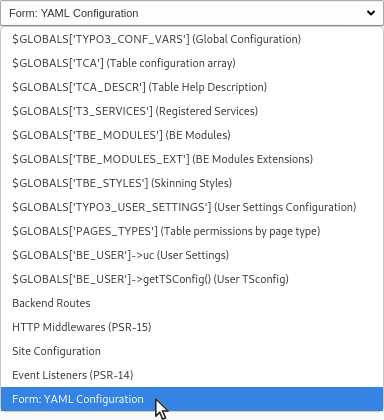
\includegraphics[width=0.70\linewidth]{ChangesForIntegrators/90052-AddYamlConfigurationToConfigurationModule.png}
			\end{figure}
		\end{column}
	\end{columns}

\end{frame}

% ------------------------------------------------------------------------------
% Feature | 88147 | Add possibility to configure the path to sitemap xslFile

\begin{frame}[fragile]
	\frametitle{Izmene za integratore}
	\framesubtitle{SEO: \texttt{Sitemap.xsl}}

	% decrease font size for code listing
	\lstset{basicstyle=\tiny\ttfamily}

	\begin{itemize}
		\item Podrazumevana putanja do fajla \texttt{Sitemap.xsl} iz sistemskog proširenja
			\texttt{EXT:seo} se može prilagoditi:

\vspace{-0.4cm}
\begin{lstlisting}
# Globally for all sitemaps:
plugin.tx_seo.config.xslFile = EXT:myext/Resources/Public/CSS/mySite.xsl

# For all sitemaps of a specific type:
plugin.tx_seo.config.<sitemapType>.sitemaps.xslFile = EXT:myext/Resources/Public/CSS/mySite.xsl

# For a specific sitemap:
plugin.tx_seo.config.<sitemapType>.sitemaps.<sitemap>.config.xslFile =
  EXT:myext/Resources/Public/CSS/mySite.xsl
\end{lstlisting}

		\item Podrazumevana putanja je:\newline
			\smaller
				\texttt{EXT:seo/Resources/Public/CSS/Sitemap.xsl}
			\normalsize

	\end{itemize}

\end{frame}

% ------------------------------------------------------------------------------
% Feature | 82062 | Progress for Reference Index update on CLI

\begin{frame}[fragile]
	\frametitle{Izmene za integratore}
	\framesubtitle{Indeks referenci}

	% decrease font size for code listing
	\lstset{basicstyle=\tiny\ttfamily}

	\begin{itemize}
		\item Tokom ažuriranja indeksa referenci za svaku tabelu je prikazan progress bar.
	\end{itemize}

	\begin{figure}
		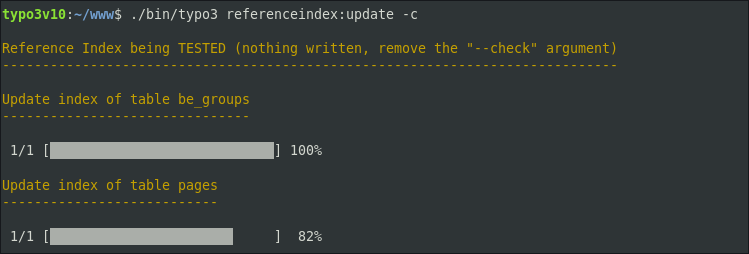
\includegraphics[width=0.85\linewidth]{ChangesForIntegrators/82062-ProgressForReferenceIndexUpdateOnCli.png}
	\end{figure}

\end{frame}

% ------------------------------------------------------------------------------
% Feature | 90425 | Add seo fields to info module

\begin{frame}[fragile]
	\frametitle{Izmene za integratore}
	\framesubtitle{Info modul}

	\begin{itemize}
		\item U Info modul su dodati SEO i Social Media detalji:\newline
			\textbf{WEB} $\rightarrow$ \textbf{Info} $\rightarrow$ \textbf{Pagetree Overview}.
	\end{itemize}

	\begin{figure}
		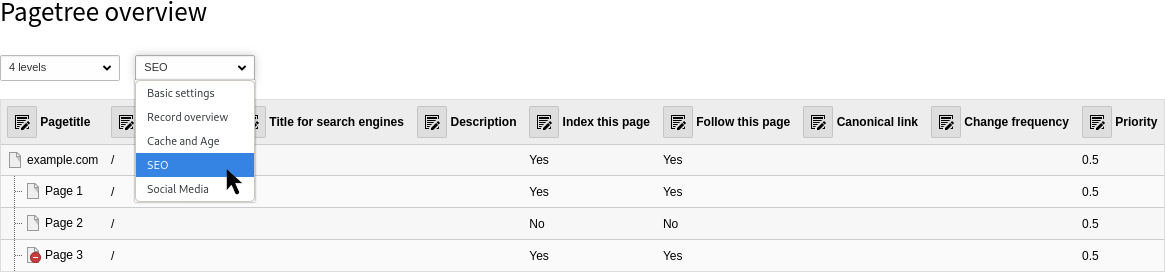
\includegraphics[width=0.85\linewidth]{ChangesForIntegrators/90425-AddSeoFieldsToInfoModule.png}
	\end{figure}

\end{frame}

% ------------------------------------------------------------------------------
% Feature | 59452 | scheduler:run command accepts multiple task options

\begin{frame}[fragile]
	\frametitle{Izmene za integratore}
	\framesubtitle{Scheduler}

	% decrease font size for code listing
	\lstset{basicstyle=\tiny\ttfamily}

	\begin{itemize}
		\item Više taskova se može izvršiti istovremeno korišćenjem opcije \texttt{-}\texttt{-}\texttt{task}
	\end{itemize}

	\begin{figure}
		
\includegraphics[width=0.85\linewidth]{ChangesForIntegrators/59452a-MultipleTasksInSchedulerCommand.png}
	\end{figure}

	\begin{itemize}
		\item Opširan izveštaj se može omogućiti sa \texttt{-}\texttt{v} i \texttt{-}\texttt{vv}
	\end{itemize}

	\begin{figure}
		
\includegraphics[width=0.85\linewidth]{ChangesForIntegrators/59452b-MultipleTasksInSchedulerCommand.png}
	\end{figure}

\end{frame}

% ------------------------------------------------------------------------------
% Feature | 90298 | Improve user info in BE User module

\begin{frame}[fragile]
	\frametitle{Izmene za integratore}
	\framesubtitle{Modul za korisnike administratorskog interfejsa}

	\begin{itemize}
		\item Novi pregled detalja korisnika administratorskog interfejsa prikazuje sve bitne podatke.
		\item Funkcionalnosti za uporedjivanje su dodata nova polja.
		\item Ova funkcionalnost sada uzima u obzir i podgrupe.
		\item Izgled ovog modula će se dodatno optimizovati.
		\item Ove izmene omogućavaju lakše uporedjivanje permisija korisnika bez potrebe
			da se prelazi na drugog korisnika.
	\end{itemize}

\end{frame}

% ------------------------------------------------------------------------------
% Feature | 89894 | Separate system extensions from 3rd-party extensions visually

\begin{frame}[fragile]
	\frametitle{Backend User Interface}
	\framesubtitle{Upravljač proširenjima}

	U upravljaču proširenja se mogu listati posebno istemska i prilagodjena proširenja.

	\begin{figure}
		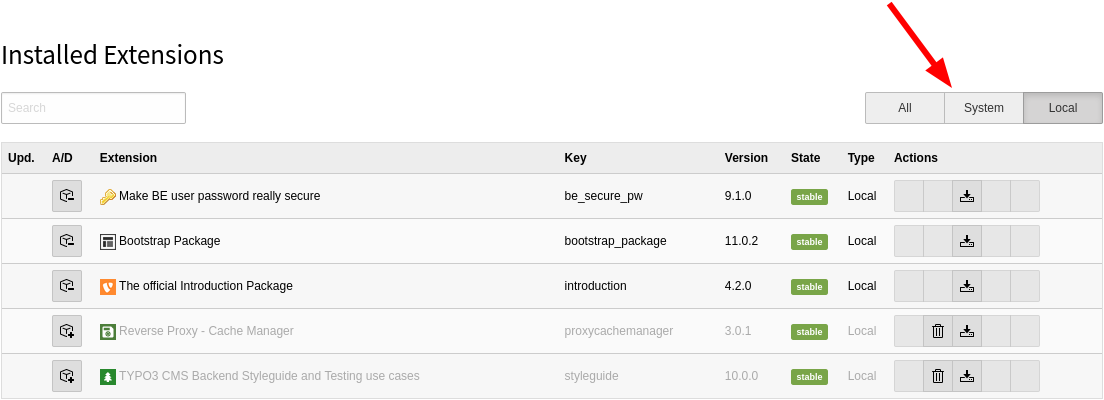
\includegraphics[width=0.9\linewidth]{BackendUserInterface/89894-SeparateSystemExtensionsFrom3rdPartyExtensionsVisually.png}
	\end{figure}

\end{frame}

% ------------------------------------------------------------------------------
% Feature | 90136 | Show application context in the Environment module

\begin{frame}[fragile]
	\frametitle{Izmene za integratore}
	\framesubtitle{Pregled okruženja}

	Kontekst aplikacije se sada prikazuje u modulu okruženja:\newline
	\textbf{ADMIN TOOLS} $\rightarrow$ \textbf{Environment} $\rightarrow$ \textbf{Environment Overview}.

	\begin{figure}
		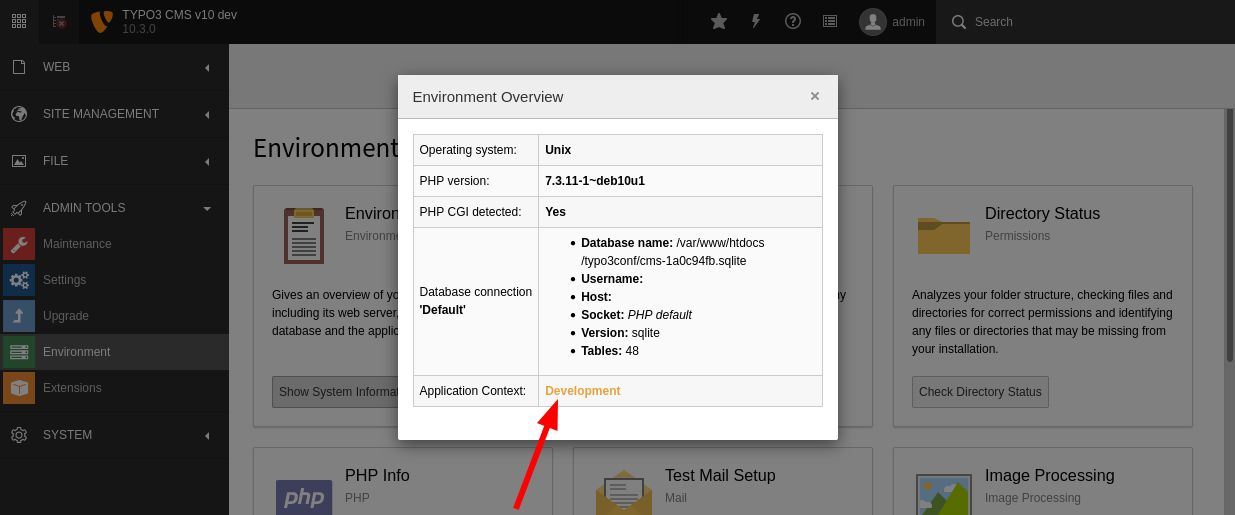
\includegraphics[width=0.9\linewidth]{ChangesForIntegrators/90136-ShowApplicationContextInTheEnvironmentModule.png}
	\end{figure}

\end{frame}

% ------------------------------------------------------------------------------
% Task | 89844 | Improve visual appearance of feature toggles

\begin{frame}[fragile]
	\frametitle{Izmene za integratore}
	\framesubtitle{Feature Toggles}

	Vizuelni prikaz za uključivanje/isključivanje funkcionalnosti je unapredjen:
	\newline\newline
	\smaller\textbf{TYPO3 < 10.3}\tabto{6cm}\textbf{TYPO3 >= 10.3}\normalsize

	\begin{figure}
		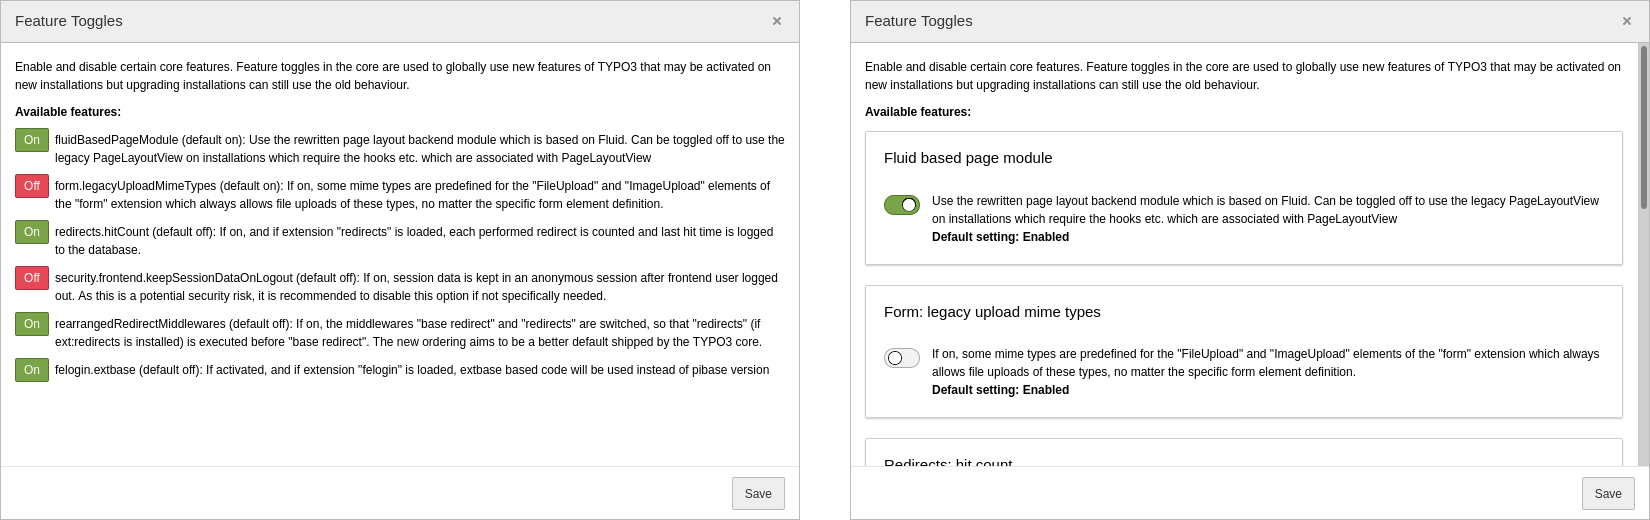
\includegraphics[width=1\linewidth]{ChangesForIntegrators/89844-ImproveVisualAppearanceOfFeatureToggles.png}
	\end{figure}

\end{frame}

% ------------------------------------------------------------------------------
% Feature | 89513 | Provide password recovery for backend users
%
%\begin{frame}[fragile]
%	\frametitle{Izmene za integratore}
%	\framesubtitle{Password Recovery Email}
%
%	\begin{itemize}
%
%		\item Password resets for backend users are only valid for 4 hours.\newline
%			This time limit is not configurable.
%		\item The function can optionally be disabled for all users or for admin users only to strengthen security.
%		\item If users share one email address, an alternative email text is used.
%		\item TCA field \texttt{be\_users.email} must not be set to \texttt{eval=email}.
%
%		\item The function only works for users, who:
%			\begin{itemize}
%				\item have an email address set,
%				\item have a password set, and
%				\item are not disabled/deleted.
%			\end{itemize}
%
%	\end{itemize}
%
%\end{frame}
%
% ------------------------------------------------------------------------------
